\section{Operations on arrays}

\subsection{Element-wise vs. matrix multiplication}
\textit{Matrix multiplication} uses \verb|*| and follows the mandatory dimension compatibility rule: if $A$ is an $m\times n$ matrix and $B$ is an $n\times p$ matrix, then \verb|C = A * B| produces an $m\times p$ matrix.
\begin{multicols}{2}
	\begin{verbatim}
		--> A = [2  1; 5  7; 9  3]
		A = [3x2 double]
		2.   1.
		5.   7.
		9.   3.
		
		--> size(A)
		ans = [1x2 double]
		3.   2.
		
		--> B = [-4  8  9;  1 7  2]
		B = [2x3 double]
		-4.   8.   9.
		1.   7.   2.
		
		--> size(B)
		ans = [1x2 double]
		2.   3.
		
		--> C = A * B
		C = [3x3 double]
		-7.    23.   20.
		-13.   89.   59.
		-33.   93.   87.
		
		--> size(C)
		ans = [1x2 double]
		3.   3.
	\end{verbatim}
\end{multicols}

\textit{Element-wise multiplication} operates on corresponding entries and uses the \verb|.*| operator. Both operands must have the same shape.
\begin{multicols}{2}
	\begin{verbatim}
	--> A = [2  1; 5  7; 9  3]
	A = [3x2 double]
	2.   1.
	5.   7.
	9.   3.
	
	--> B = [-4  8;  9  1;  7  2]
	B = [3x2 double]
	-4.   8.
	9.   1.
	7.   2.
	
	--> C = A .* B
	C = [3x2 double]
	-8.    8.
	45.   7.
	63.   6.
	
	--> D = [-4  8  9;  1  7  2]
	D = [2x3 double]
	-4.   8.   9.
	1.   7.   2.
	
	--> A .* D
	Operator .*: Wrong dimensions for
		operation
	[3x2] .* [2x3], same dimensions
		expected.
	\end{verbatim}
\end{multicols}

\subsection{Matrix computations}

\subsubsection{Transpose}
The transpose of a matrix is another matrix whose rows and columns are swapped. In Scilab, the transpose of a matrix \verb|A| is obtained by the \verb|'| operator, i.e. \verb|A'| is conjugate transpose of \verb|A|.
\begin{multicols}{2}
	\begin{verbatim}
	--> A = [2  1; 5  7; 9  3]
	A = [3x2 double]
	2.   1.
	5.   7.
	9.   3.
	
	--> A'
	ans = [2x3 double]
	2.   5.   9.
	1.   7.   3.
	
	--> B = [-4  8  9  1  7]
	B = [1x5 double]
	-4.   8.   9.   1.   7.
	
	--> B'
	ans = [5x1 double]
	-4.
	8.
	9.
	1.
	7.
	\end{verbatim}
\end{multicols}

\subsubsection{Determinant}
The determinant of a matrix is a single scalar value computed from a square matrix. In Scilab, the determinant of a square matrix \verb|A| is obtained by the \verb|det()| function.
\begin{multicols}{2}
	\begin{verbatim}
	--> A = [3  4  6; 7  -1  2; 8  5  9]
	A = [3x3 double]
	3.   4.   6.
	7.  -1.   2.
	8.   5.   9.
	
	--> size(A)
	ans = [1x2 double]
	3.   3.
	
	--> det(A)
	ans = 
	13.000000
	
	--> B = [2  1; 5  7; 9  3]
	B = [3x2 double]
	2.   1.
	5.   7.
	9.   3.
	
	--> size(B)
	ans = [1x2 double]
	3.   2.
	
	--> det(B)
	det: Wrong type for input argument #1:
	Square matrix expected.
	\end{verbatim}
\end{multicols}

\subsubsection{Inverse}
The inverse of a square matrix exists only if it is non-singular, i.e. its determinant exists. In Scilab, the matrix inverse is computed with the \verb|inv()| function for a square, non-singular matrix.
\begin{multicols}{2}
	\begin{verbatim}
	--> A = [3 4 6; 7 -1 2; 8 5 9]
	A = [3x3 double]
	3.   4.   6.
	7.  -1.   2.
	8.   5.   9.
	
	--> det(A)
	ans = 
	13.000000
	
	--> inv(A)
	ans = [3x3 double]
	-1.4615385  -0.4615385   1.0769231
	-3.6153846  -1.6153846   2.7692308
	3.3076923   1.3076923  -2.3846154
	
	--> B = [1  2; 2  4]
	B = [2x2 double]
	1.   2.
	2.   4.
	
	--> det(B)
	ans = 
	0.
	
	--> inv(B)
	inv: Problem is singular.
	\end{verbatim}
\end{multicols}

\subsubsection{Eigenvalues: solving linear systems}
For a square matrix $\boldsymbol{A}$, a non-zero vector $\boldsymbol{v}$ is called an eigenvector and the number $\lambda$ is called the corresponding if they satisfy the following matrix equation
\begin{align*}
	\boldsymbol{Av}&=\lambda\boldsymbol{v}
\end{align*}
Geometrically, an eigenvector points in a direction that the matrix does not rotate, i.e. it is only stretched or shrunk by the factor $\lambda$.

Eigenvalues and eigenvectors are useful for finding natural modes, studying stability, and simplifying matrix problems; they are usually computed with software and checked by confirming that $\boldsymbol{Av}$ is approximately equal to $\lambda\boldsymbol{v}$.

In Scilab, the eigenvectors and eigenvalues are obtained using the \verb|spec()| function. This function returns two matrices -- one containing the eigenvectors as columns, and the other containing the eigenvalues as diagonals.
\begin{multicols}{2}
	\begin{verbatim}
	--> A = [2 1; 1 2]
	A = [2x2 double]
	2.   1.
	1.   2.
	
	--> [V, D] = spec(A);
	
	--> V
	V = [2x2 double]
	-0.7071068   0.7071068
	0.7071068   0.7071068
	
	--> D
	D = [2x2 double]
	1.   0.
	0.   3.
	
	--> disp("Eigenvalues (diagonal entries
	of D):"), disp(diag(D));
	"Eigenvalues (diagonal entries of D):"
	1.
	3.
	
	--> disp("Eigenvector matrix V (columns
	are eigenvectors):"), disp(V);
	"Eigenvector matrix V (columns
	are eigenvectors):"
	-0.7071068   0.7071068
	0.7071068   0.7071068
	\end{verbatim}
\end{multicols}

\subsection*{\MakeUppercase{Exercises}}
\begin{enumerate}
	\item As shown in the figure below, a system of three particles of masses $m_1=4.1$ kg, $m_2=8.2$ kg and $m_3=4.1$ kg is initially at rest. The particles are each acted on by different net external forces, which have magnitudes $F_1=6$ N, $F_2=12$ N and $F_3=14$ N, whose directions are also shown in the figure. Write a Scilab program to compute the magnitude of the acceleration of the center of mass.
	\begin{figure}[!h]
		\centering
		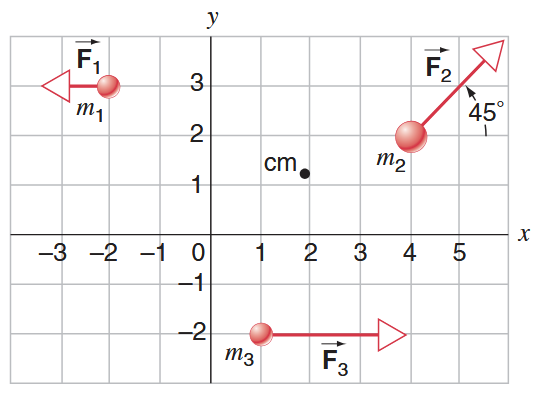
\includegraphics[width=0.4\linewidth]{figures/fig_sys-of-particles.png}
	\end{figure}
	
	\item Given the matrix $\boldsymbol{A}=\begin{bmatrix}
		{4} & {1} & {2} \\
		{0} & {3} & {-1} \\
		{1} & {0} & {2}
	\end{bmatrix}$
	\begin{enumerate}[a)]
		\item Write the Scilab command to compute $|\boldsymbol{A}|$ and state whether $\boldsymbol{A}$ is invertible.
		\item  If invertible, write the Scilab command to compute $\boldsymbol{A}^{-1}$.
		\item Write the Scilab command to compute the eigenvalues of $\boldsymbol{A}$.
	\end{enumerate}
\end{enumerate}